\appendix
\addcontentsline{toc}{section}{Appendici}
\section*{Appendici}
\section{Resoconto delle attività di verifica}
La seguente sezione riporta il resoconto delle attività di verifica svolte prima di ciascuna delle quattro revisioni stabilite dal committente (Revisione dei Requisiti, Revisione di Progettazione, Revisione di Qualifica e Revisione di Accettazione).
Al termine di ogni revisione, il committente segnalerà le problematiche riscontrate attraverso una valutazione globale dell'andamento del progetto ed una dettagliata per ciascun documento; questo aiuterà il gruppo a eliminare problemi e criticità nel progetto per poi procedere su una base verificata e il più possibile corretta.

\subsection{Revisione dei Requisiti}
In questa sezione vengono riportati gli esiti delle metriche relative ai processi e delle metriche relative ai documenti.
\subsubsection{Qualità di processo}
 
\paragraph{Esiti metriche di processo} \Spazio
\renewcommand{\arraystretch}{1.5}
\begin{table}[H]
	\begin{center}
		\begin{tabular}{|c|c|c|}
			\hline
			\rowcolor{title_row}
			\textbf{\color{title_text}{Documento}} & \textbf{\color{title_text}{Valore ottenuto}} & \textbf{\color{title_text}{Esito}} \\
			\hline
			{Schedule Variance} & {} & {Superato}\\	
			\hline
			{Budget Variance} & {} & {Superato}\\	
			\hline
		\end{tabular}
	\caption[Esiti metriche di processo, Analisi]{Esiti derivanti dall'applicazione delle metriche di processo}	
	\label{tabella: esiti derivanti dall'applicazione delle metriche di processo}
	\end{center}
\end{table}

\renewcommand{\arraystretch}{1}
\paragraph{Dettaglio delle verifiche tramite analisi} \Spazio
Il grafico rappresentante l'applicazione del metodo PDCA della fase di Analisi è:
\begin{figure} [H]
	\centering
	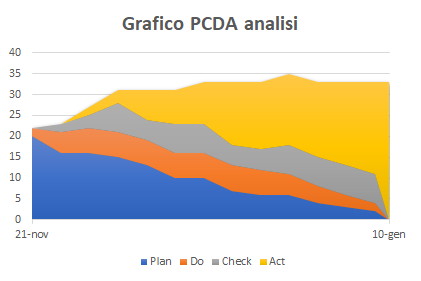
\includegraphics[scale=1]{Img/Grafico_PDCA}
	\caption{Grafico del metodo PDCA, fase di Analisi}\label{}
\end{figure}
Dal grafico possiamo estrapolare che:
\begin{itemize}
	\item Si notato alcuni mutamenti dei processi pianificati, dovuti ad errori di pianificazione dati dalla poca esperienza del gruppo di lavoro;
	\item Si può notare come il gruppo abbia cercato di rendere omogenea nel tempo l'avanzamento dei processi, alcuni rallentamenti sono dovuti alla sovrapposizione degli impegni
	universitari dei componenti del gruppo con la realizzazione del progetto. Nel complesso si vede come l'omogeneità è stata abbastanza rispettata.
\end{itemize}
\subsubsection{Qualità di prodotto}
\paragraph{Indice di Gulpease} \Spazio
Vengono qui riportati i valori dell'indice Gulpease per ogni documento durante la fase
di Analisi. Un documento è considerato valido soltanto se rispetta le metriche descritte
su 4.1.
\renewcommand{\arraystretch}{1.5}
\begin{table}[H]
\begin{center}
\begin{tabular}{|c|c|c|}
\hline
\rowcolor{title_row}
\textbf{\color{title_text}{Documento}} & \textbf{\color{title_text}{Valore indice}} & \textbf{\color{title_text}{Esito}} \\
\hline
	\emph{Piano di Progetto v1.0.0} & {55.49} & {Superato}\\
\hline
	\emph{Norme di Progetto v1.0.0} & {54.54} & {Superato}\\
\hline
	\emph{Analisi dei Requisiti v1.0.0} & {58.80} & {Superato}\\
\hline
	\emph{Piano di Qualifica v1.0.0} & {53.98} & {Superato}\\
\hline
	\emph{Studio di Fattibilità v1.0.0} & {50.77} & {Superato}\\
\hline
	\emph{Glossario v1.0.0} & {51.66} & {Superato}\\
\hline
\end{tabular}
\caption[Esiti verifica documenti, Analisi]{Esito verifica documenti}
\label{tabella:verifica documenti}
\end{center}
\end{table}
\renewcommand{\arraystretch}{1}

Dalla tabella si può notare come tutti gli indici Gulpease dei documenti rientrino nei vincoli dati. Per questo motivo i documenti redatti hanno raggiunto la leggibilità desiderata.

\paragraph{Gunning fog index} \Spazio

\subsubsection{Dettaglio dell'esito della revisione}
\begin{itemize}
	\item\emph{Norme di Progetto}: sono state effettuate le integrazioni richieste ed è stata aggiornata la struttura del documento in modo da rispettare gli stessi standard per ogni sezione.\\
	La sottosezione relativa alla verifica è stata opportunamente aggiornata in modo da contenere le nuove metriche inserite e le vecchie metriche erroneamente presenti nel \emph{Piano di Qualità v1.0.0}.	\item\emph{Analisi dei Requisiti}: al documento sono state attuate le opportune modifiche suggerite. Alcuni casi d'uso sono stati leggermente rivisti ed è stato introdotto un caso d'uso più generico per ogni agglomerato di azioni con attitudini simili. Ciò ha portato ad un importante cambiamento del caso d'uso principale. 	
	\item\emph{Piano di Progetto}: sono state fatte alcune verifiche nell'uso di alcuni termini e standard come consigliato dal committente. Sono stati aggiunte le opportune motivazioni e spiegazioni nelle scelte effettuate. La presentazione dei contenuti è stata rivista in modo da renderla più efficace.
	\item\emph{Piano di Qualifica}: il documento è stato profondamente rivisto per struttura e contenuti secondo le specifiche del committente. \\
	Le specifiche degli standard utilizzati sono stati spostati in appendice alle \emph{Norme di Progetto}, come anche la descrizione delle metriche hanno trovato posto nello stesso documento. Le specifiche dei test sono state trasferite in appendice al documento. Infine, la strategia generale per la verifica ha assunto un ruolo centrale nella specifica degli obiettivi di qualità di processo e prodotto. 
\end{itemize}
\pagebreak

\subsection{Revisione di Progettazione}
In questa sezione vengono riportati gli esiti delle metriche relative ai processi e delle metriche relative ai documenti.
\subsubsection{Qualità di processo}

\paragraph{Esiti metriche di processo} \Spazio
\renewcommand{\arraystretch}{1.5}
\begin{table}[H]
	\begin{center}
		\begin{tabular}{|c|c|c|}
			\hline
			\rowcolor{title_row}
			\textbf{\color{title_text}{Documento}} & \textbf{\color{title_text}{Valore ottenuto}} & \textbf{\color{title_text}{Esito}} \\
			\hline
			{Schedule Variance} & {} & {Superato}\\	
			\hline
			{Budget Variance} & {} & {Superato}\\	
			\hline
		\end{tabular}
		\caption[Esiti metriche di processo, Analisi]{Esiti derivanti dall'applicazione delle metriche di processo}	
		\label{tabella: esiti derivanti dall'applicazione delle metriche di processo}
	\end{center}
\end{table}

\paragraph{Maturità dei processi} \Spazio
Come riportato nella sezione 2.1.6, il gruppo adotta l'approccio a maturità di processo. Il livello di maturità assume valori da 1 a 5.
\renewcommand{\arraystretch}{1.5}
\begin{table}[H]
	\begin{center}
		\begin{tabular}{|c|c|c|}
			\hline
			\rowcolor{title_row}
			\textbf{\color{title_text}{Processo}} & \textbf{\color{title_text}{Livello di maturità}} & \textbf{\color{title_text}{Considerazioni}} \\
			\hline
			{Pianificazioni e controllo} & {} & {}\\	
			\hline
			{Gestione dei rischi} & {} & {}\\	
			\hline
			{Gestione dei test} & {?} & {?}\\	
			\hline
			{Versionamento e build} & {} & {}\\	
			\hline
			
		\end{tabular}
		\caption[Maturità dei processi, Analisi]{Maturità ei processi e considerazioni}	
		\label{tabella: considerazioni sulla maturità dei processi raggiunta}
	\end{center}
\end{table}


\renewcommand{\arraystretch}{1}
\paragraph{Dettaglio delle verifiche tramite analisi} \Spazio
Il grafico rappresentante l'applicazione del metodo PDCA della fase di Analisi è:
\begin{figure} [H]
	\centering
	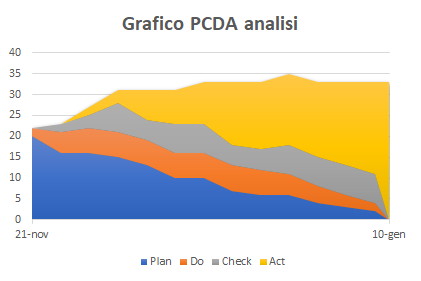
\includegraphics[scale=1]{Img/Grafico_PDCA}
	\caption{Grafico del metodo PDCA, fase di Analisi}\label{}
\end{figure}
Dal grafico possiamo estrapolare che:
\begin{itemize}
	\item Si notato alcuni mutamenti dei processi pianificati, dovuti ad errori di pianificazione dati dalla poca esperienza del gruppo di lavoro;
	\item Si può notare come il gruppo abbia cercato di rendere omogenea nel tempo l'avanzamento dei processi, alcuni rallentamenti sono dovuti alla sovrapposizione degli impegni
	universitari dei componenti del gruppo con la realizzazione del progetto. Nel complesso si vede come l'omogeneità è stata abbastanza rispettata.
\end{itemize}
\subsubsection{Qualità di prodotto}
\paragraph{Indice di Gulpease} \Spazio
Vengono qui riportati i valori dell'indice Gulpease per ogni documento durante la fase
di Analisi. Un documento è considerato valido soltanto se rispetta le metriche descritte
su 4.1.
\renewcommand{\arraystretch}{1.5}
\begin{table}[H]
	\begin{center}
		\begin{tabular}{|c|c|c|}
			\hline
			\rowcolor{title_row}
			\textbf{\color{title_text}{Documento}} & \textbf{\color{title_text}{Valore indice}} & \textbf{\color{title_text}{Esito}} \\
			\hline
			\emph{Piano di Progetto v1.0.0} & {55.49} & {Superato}\\
			\hline
			\emph{Norme di Progetto v1.0.0} & {54.54} & {Superato}\\
			\hline
			\emph{Analisi dei Requisiti v1.0.0} & {58.80} & {Superato}\\
			\hline
			\emph{Piano di Qualifica v1.0.0} & {53.98} & {Superato}\\
			\hline
			\emph{Studio di Fattibilità v1.0.0} & {50.77} & {Superato}\\
			\hline
			\emph{Glossario v1.0.0} & {51.66} & {Superato}\\
			\hline
		\end{tabular}
		\caption[Esiti verifica documenti, Analisi]{Esito verifica documenti}
		\label{tabella:verifica documenti}
	\end{center}
\end{table}
\renewcommand{\arraystretch}{1}

Dalla tabella si può notare come tutti gli indici Gulpease dei documenti rientrino nei vincoli dati. Per questo motivo i documenti redatti hanno raggiunto la leggibilità desiderata.

\paragraph{Gunning fog index} \Spazio

\section{Specifiche dei test}
Questa appendice contiene le specifiche relative ai vari test pianificati. Verrà redatta una volta presente la necessità di eseguire tali test.
